We suggest developing an engaging ``canvas''  for authoring e-learning 
modules, taking cues from 
\begin{CJK}{UTF8}{min}RPGツクール\end{CJK}\footnote{\url{http://www.rpgmakerweb.com/}}, 
Game Maker\footnote{\url{https://www.yoyogames.com/studio}}, and other similar 
software that succeed in take advantage of an intuitive interface with a 
capacious featureset.

By ``canvas'' (or ``scene graph''), we mean an easy-to-learn system of widgets 
and composite stores (with rich content), and flows connecting them together 
to a cohesive system. The widgets would initially be H5P modules.

An example of such a system might be a test leveraging media like GNU 
Mediagoblin, Youtube, NRK, Twitter, and Nasjonal Digital 
Læringsarena\footnote{\url{http://ndla.no/}} to showcase the issue at hand by 
embedding video and articles, etc., before testing the user's comprehension at 
the end with an H5P quiz. Such a system is shown in 
Figure~\ref{fig:younrkquiz}. Thus, the student-come-software-developer is able 
to prove their comprehension of multimedia (as mandated by the curriculum), 
and other students are permitted to take part in the learning experience.
Incentives for doing so might be given by the teacher, or by arranging 
collaborations that invite the students to share their best ideas.

\begin{figure}[H]
    \centering
    \begin{scale}{0.1}
        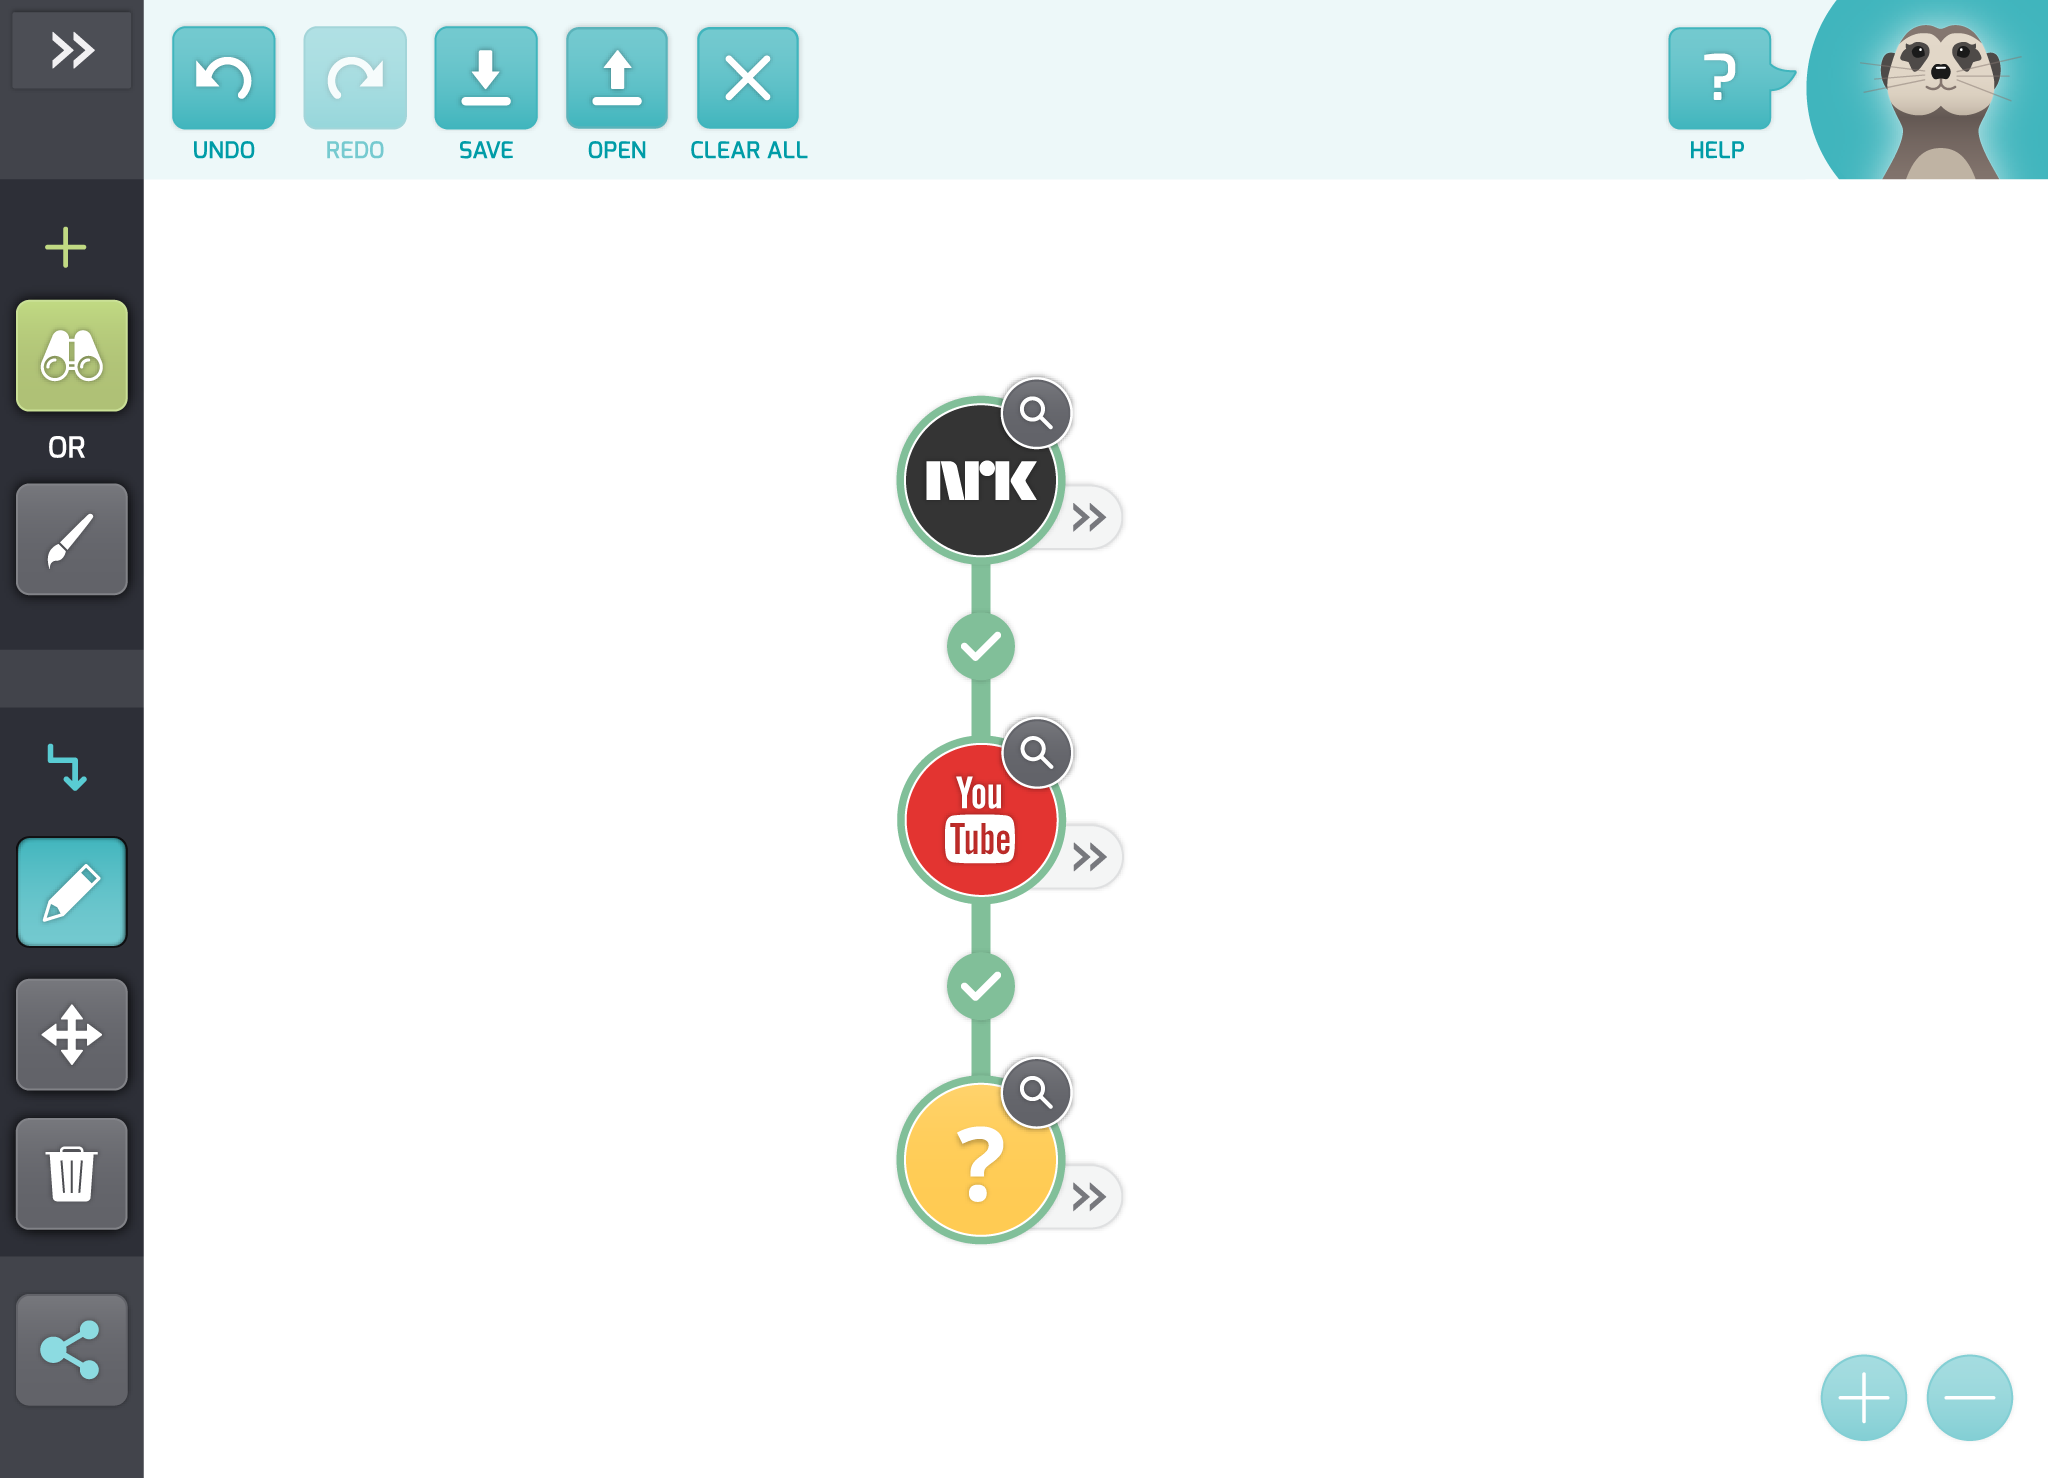
\includegraphics{fig/younrkquiz.png}
    \end{scale}
    \caption{A system where the user watches a YouTube video, then reads an 
   article on NRK, and finally does a quiz}
\label{fig:younrkquiz}
\end{figure}

Taking cue from Minecraft, we also propose another viable incentive: The 
student is provided with ready-made canvases with actors and stores made by 
other users, and encouraged to make the application perform certain actions 
(``gamification''). This is akin to the redstone system found in Minecraft, 
where even young users are able to construct discrete logic circuits providing 
useful functionality like opening doors, or switching on 
lights\cite{brand2013crafting}.

Consequently, we have customisable flows between widgets. They may be 
customised initially via simple if-expressions on the form $if$ $\chi$ $then$ 
$\alpha$, $else$ $\beta$, where e.g. $\chi=$ 80\% completion rate, and 
$\alpha=$ an H5P memory game, and $\beta=$ an H5P quiz. An example of the 
conditions dialogue is shown in Figure~\ref{fig:conditions}.

Through use of our canvas, we eliminate the BOP by liberating and empowering 
it to make its own user experience. As an added bonus, our canvas may spark 
some latent creative souls, or inspire technological awareness and interest. 
In our increasingly computerised society, this is in itself a noble cause. 

Thus, this canvas might prove to be a force for bridging the gap between just 
being a computer user, and having a promising future career in computer 
software. While Computing At 
School\footnote{\url{http://www.computingatschool.org.uk/}} have had great 
success in the UK, there is as of today no readily-available path for 
acquiring the advanced knowledge needed to develop modern systems given the 
current education system in Norway. Grassroots organisations such as Lær Kidsa 
Koding\footnote{\url{http://www.kidsakoder.no/}} are doing good work, but have 
yet to strongly influence the education system. If our canvas is picked up by 
prominent e-learning providers like Nasjonal digital læringsarena we can 
liberate and empower users through direct action, circumventing bureaucracy.

In addition to users teaching themselves technology, they also teach 
themselves the curriculum more effectively. The student becomes the teacher, 
and we achieve learning by teaching, an often sought-after method of 
reinforced learning. By only being e-learning module \emph{users}, students 
are limited to learning through observation, experimentation, and (to some 
extent) mistakes. Learning through teaching offers advantages not possible to 
fully realise through either of these; advantages that won't manifest if the 
student is exclusively relying on an external 
teacher\cite{cortese2005learning}.

\begin{figure}[H]
    \centering
    \begin{scale}{0.1}
        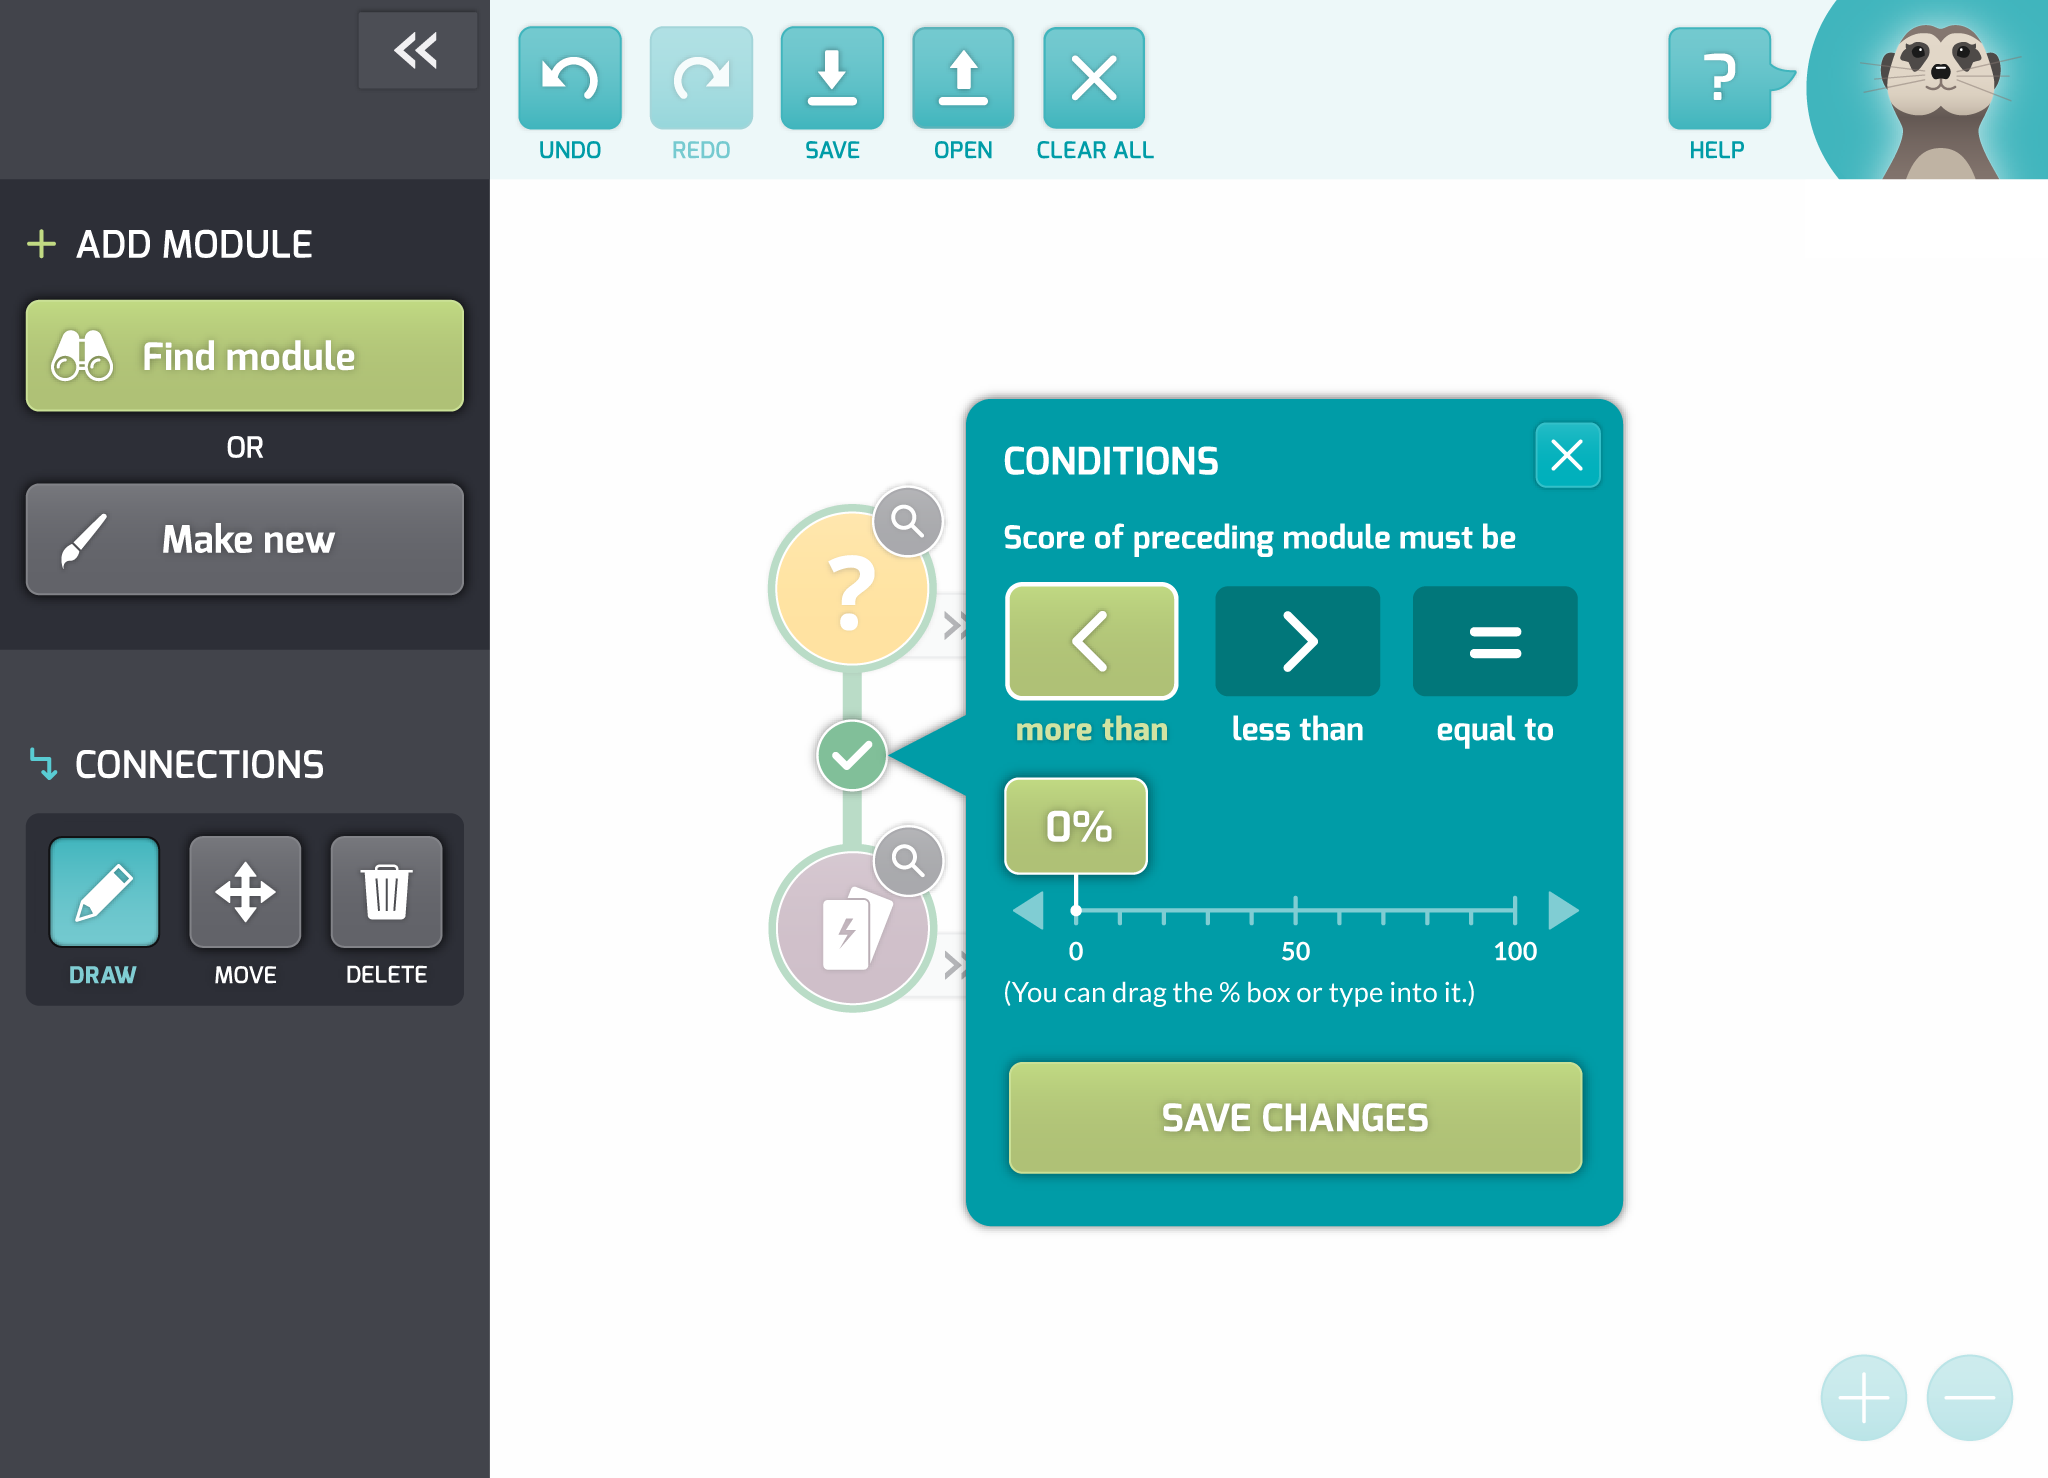
\includegraphics{fig/conditions.png}
    \end{scale}
    \caption{A dialogue for tweaking conditional flow}
\label{fig:conditions}
\end{figure}

Our canvas makes composing e-learning modules intuitive for non-technical 
users and at the same time powerful enough to entice power users and 
established e-learning module authors. Consequently, the target demographic of 
our canvas is not limited to the BOP, but extends to include current 
e-learning module authors.

To further underline our empowering of the BOP, we make sharing of works very 
simple, and make it equally simple to author derivatives (forks) and 
meta-works (collections). Incentive for sharing your work, and improving or 
remixing the work of others is provided through gamification of the canvas. As 
an example, there may be a reward system for users whose modules are often 
remixed, and for users who make an improvement to a module that then gets 
integrated back into the original module itself. These rewards are then 
presented in a positive and motivating way to the user, as shown in 
Figure~\ref{fig:rewards}.

\begin{figure}[H]
    \centering
    \begin{scale}{0.1}
        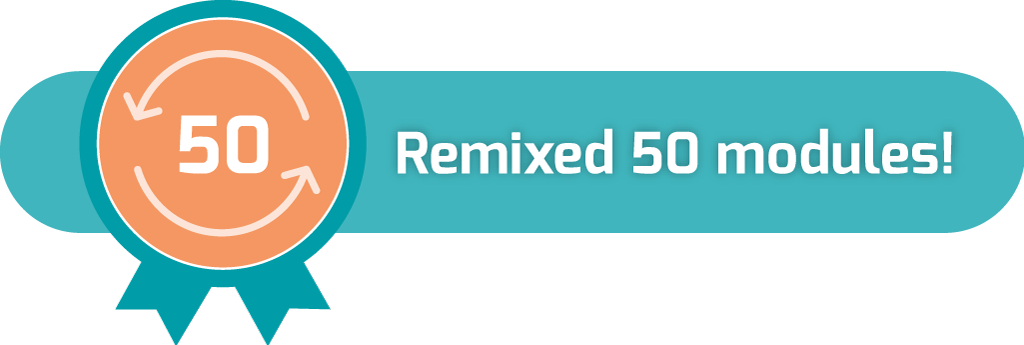
\includegraphics{fig/rewards.png}
    \end{scale}
    \caption{A reward for positive behaviour}
\label{fig:rewards}
\end{figure}

With gamification, we can also help ensure high quality modules. With a rating 
system and achievements for obtaining a high rating, we realise a 
self-regulating community.

Initially we aim to support authoring H5P modules, focussing our development 
at H5P integration. But with a good modular design we can extend our canvas to 
support other standards as well in the future. We also want to support 
embedding of things like videos and news articles. Lastly, careful attention 
must be paid to the application programming interface, so that it is easy for 
future e-learning modules to support our system.
